%\documentclass[a4paper]{article}
\documentclass[17pt]{extarticle}
\usepackage{polyglossia}
\usepackage{textcomp}
\usepackage{epigraph, varwidth}
\renewcommand{\epigraphsize}{\small}
\setlength{\epigraphwidth}{0.9\textwidth}
\usepackage{color, colortbl}
\usepackage{xcolor}
\usepackage{graphicx}
\usepackage{tabularx} % in the preamble
\usepackage[margin=15mm]{geometry}
\usepackage{hyperref}
\hypersetup{
    backref=true,
    citecolor=magenta,
    colorlinks=true,
    linkcolor=blue,
    filecolor=magenta,
    urlcolor=cyan,
}
\urlstyle{same}
\setmainfont[Scale=0.9]{Noto Serif}
\setotherlanguages{marathi}
\newfontfamily\marathifont[Mapping=velthuis-sanskrit,Script=Devanagari,Language=Marathi]{Noto Serif Devanagari}
% define acronyms https://tex.stackexchange.com/a/73681/64425
\usepackage{xspace}
\newcommand*{\subjbio}{AP Biology\textregistered\xspace}
\newcommand*{\subjchem}{AP Chemistry\xspace}
\newcommand*{\subjsans}{Samskitam (\textmarathi{sa.msk.rtam})\xspace}
\newcommand*{\subjmath}{Math Exploration\xspace}
\newcommand*{\subjcs}{Computer Science\xspace}
% define acronyms https://tex.stackexchange.com/a/73681/64425
% control hyphenation: https://tex.stackexchange.com/a/177179/64425
\tolerance=1
\emergencystretch=\maxdimen
\hyphenpenalty=10000
\hbadness=10000
% control hyphenation: https://tex.stackexchange.com/a/177179/64425
% make sure ~ as non-breaking space doesn't interfere with velthuis-sanskrit mapping
\edef~{\string~}
\begin{document}
% ....
\begin{center}
\begin{minipage}{.4\textwidth}
%\centering
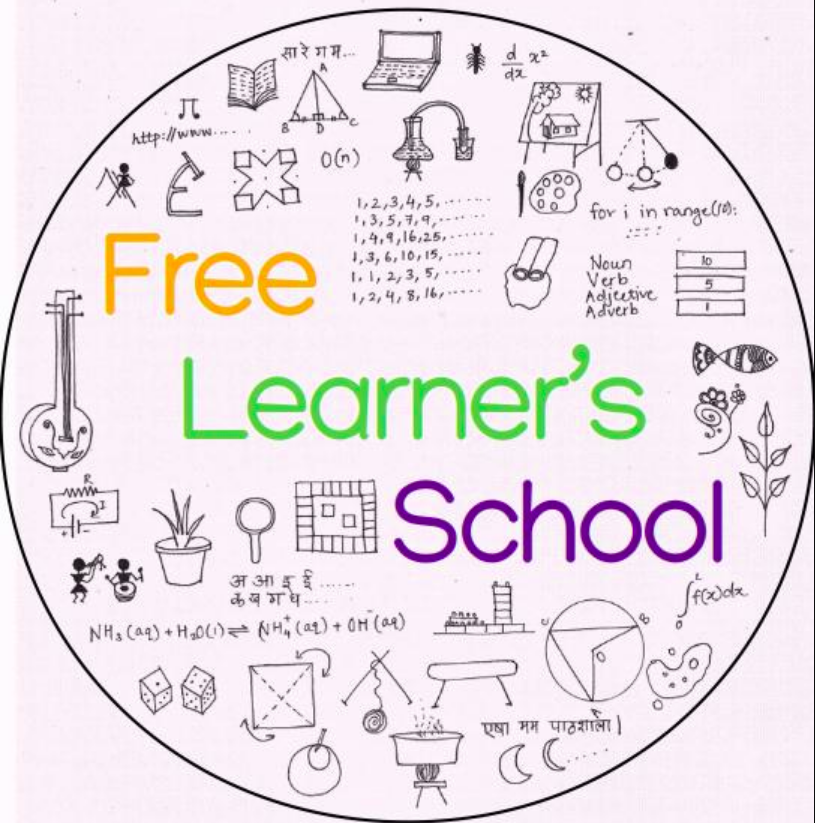
\includegraphics[height=2cm]{fls-school-logo.png}
\end{minipage}
\end{center}
\centering
{\Large \underline{Report Card}}
\begin{tabularx}{\textwidth}{lX}
Name: &  Apoorv Mhaswade\\
Grade: & Ten \\
Academic Year: &2020-21  \\
\end{tabularx}
\vspace{10mm}
\begin{tabularx}{\textwidth}{|X|l|l|}
\hline
  \textbf{Subject} & \textbf{Instructor} & \textbf{Grade/Score} \\
\hline
\subjbio &
Kedar Mhaswade&
\textcolor{magenta}{\textbf{5/5}}
\\
\hline
\subjchem &
Kedar Mhaswade&
\textcolor{magenta}{\textbf{5/5}}
\\
\hline
\subjsans&
Kedar Mhaswade&
\textcolor{magenta}{\textbf{92/100}}
\\
\hline
\subjmath&
Deepa Joshi and Kedar Mhaswade&
\textcolor{magenta}{\textbf{A-}}
\\
\hline
\subjcs &
Kedar Mhaswade &
\textcolor{magenta}{\textbf{A-}}
\\
\hline
\end{tabularx}
\underline{Comments (With Constructive Feedback)}
\begin{enumerate}
\item \textbf{\subjbio}. Apoorv decided to do AP Biology \textbf{on his own} this year. This was a bold decision given that none of his \emph{steachers\footnote{A teacher who is a student of the subject matter to be taught.}} were familiar with Biology. He took great interest in the molecular biology of the cell, biological macromolecules and their basic chemistry, genetics, evolution, ecology, and the introduction to plant and human anatomy. He worked hard, studied the OpenStax \cite{openstax-bio} book, referred to YouTube and Khan Academy when needed, and referred to several scientific writings in Biology (notably Dobzhansky's ``Nothing in Biology Makes Sense except in the Light of Evolution'' \cite{dobz}, Sturtevant's ``Introduction to Genetics'' \cite{sturt}). 

Free-response questions in Biology are tough and you require a breadth of knowledge and an ability to connect disparate pieces of knowledge to predict something with confidence. He did this successfully and he was awarded for his efforts. He took the AP\textregistered exam at 9.30 p.m. India time on 11 June 2021. Initially he was nervous, but when the results came in the first week of August 2021, he was overjoyed! We are very proud of his success in AP\textregistered Biology.

One criticism of ``exam-oriented'' learning is that when the exams are over, the students' exploration or curiosity also stops, at least temporarily. We have tried to address this problem by being in the vicinity of knowledge. One thing he could do is to motivate other, younger kids to talk about Biology. We don't even mind if he took up teaching 8th or 9th graders in the neighborhood, with a view that when one teaches at least two learn. He should try to keep up-to-date with his interests in cell biology and genetics. It is going to be challenging given that he'd study other subjects next year, but we hope that he finds avenues to keep his interest in Biology. He could, for example, take up reading a fresh biography of a pioneering scientist like Jennifer Doudna \cite{doudna} or take up a course, like the one offered by Prof. Ben Langmead, on Coursera \cite{langmead} (this is especially useful given his interest in computing).

It is also important that we do experiments. It has been challenging to create a lab environment at a home-school, especially in a pandemic year. But we should (will?) give it a try. One plan is to use the microscope well. We bought a light microscope last year and Apoorv showed great interest initially, but one must admit that the interest dwindled down as time passed and exam pressure increased. If you look at many scientists' careers, however, you will realize that they turned to science only by the urge of studying nature through experiments (at times crazy experiments). Therefore I hope that we will give a try to some experiments from Thompson and Thompson's \cite{thompsbio} DIY Science book.

\item \textbf{\subjchem}. Apoorv has always been attracted to Chemistry. This year, he truly enjoyed Chemistry 2e \cite{openstax-chem}. He was in a position to sort of reintroduce himself to the Periodic Table. He took enormous interest in Atoms and Molecules, Introduction to Quantum Chemistry, Theories of Atomic, Molecular, and Ionic Bonds, Phases of Matter, Solutions and Colloids, Reaction Stoichiometry, Reaction Kinematics, Chemical Equilibria, Thermodynamics, and Electrochemistry.  His notes \cite{chem-notes} are thorough, comprehensive, and readable (although incomplete).
    
Doing all of this mostly \textbf{on one's own} is quite remarkable. He thought he'd do well in the Chemistry AP\textregistered exam, but he was rather unsure of a score of $5/5$. He was overjoyed when he learned of the perfect score.

Of course, there is a lot to learn beyond this introductory course of college chemistry. What is true of Biology is also true of Chemistry. He should plan to spend some time performing Chemistry experiments. [We] Hope he finds avenues to keep the ``keen interest in Chemistry'' candle burning. Continue reading the life and work of people like Linus Pauling. And yes, please read the great G. N. Lewis's classic paper, The Atom and the Molecule \cite{a-m} from 1916!

\item \textbf{\subjsans}. Apoorv expressed interest in learning the great Indian language, Samskitam (also written as \textmarathi{sa.msk.rtam}). His interest is mainly from the point of view of melodious verses and grammar. This is definitely a great start. He opted for the examinations by Samskrita-Bharati in Bangalore, India. Of the four examinations that they give (for remote learners via mail), in February 2021, he took the first examination called \emph{Pravesha} (also written as \textmarathi{prave"sa}) which literally means \emph{entrance}.

Although the book for this examination is pretty ``exam-oriented''. The students are expected to commit things to short-term memory and regurgitate the material on the day of examination. Against such a backdrop, however, Apoorv showed keen interest in learning the language, its scripts, its verses, and basic parts of its grammar. We also developed a system to analyze the meanings of those verses.

He mastered the Devanaagarii (also written as \textmarathi{devanaagarii}) script and wrote his exam in that script from 10 am - 1.00 pm on 28 February 2021. We are very happy about the score he achieved. He has expressed interest in doing it further. This is just the beginning of his learning of this great language of India. 

\item \textbf{\subjmath}. We wanted Apoorv to enjoy the mathematics for interested high school students. We found ``Essence of Mathematics'' by Borovik and Gardiner \cite{e-m} that is my (Kedar Mhaswade) personal favorite. He started well on this book, however, as the pressure of other exams increased, this took a backseat. Its priority reduced and we could not do it any further. I am a bit disappointed that Apoorv did not return to the book or the problems from it when time became available. Mathematical exploration is a never-ending process and one may be able to more easily find time for it during high school. Alas, this has not been possible.
        
One suggestion we have for Apoorv is to return to problems in mathematics. This book is a real gem. If you can find time to solve many of them, we assure you that your time would be spent well. Please consider doing it in spite of your other commitments (which you should fulfill). You leave something to be desired here!

        One really interesting thing Apoorv and Deepa Joshi attempted this year was the ``Inquiry-Base Learning'' (IBL) approach to mathematics (See \cite{jiblm}). This approach, developed mainly by the mathematician and professor of mathematics, Robert Lee Moore. This approach has come to be known as the Moore Method \cite{rlm}. They chose to do Precalculus using the Inquiry-Based Learning and we are happy to report that he enjoyed it very much! We wish he takes up more modules and courses from the website.

\item \textbf{\subjcs}. Since his 5th grade, Apoorv has been a Linux user and has taken interest in Computer Science. It is like his first love and it was quite evident when he completed his AP\textregistered Computer Science exam in his ninth grade. We continued our exploration and picked up Eric Roberts's ``Thinking Recursively'' \cite{recur} which beautifully brings out the essence of recursion. Apoorv did many programming problems really well. He took his assignments seriously \cite{gh-vw}.

It was not required by any exam that Apoorv sets aside time for doing recursive programs this year. For this, we really admire him since it was a ``labor of love'' for him. We encourage him to complete the recursive data structures as soon as possible so that he can understand how the data structures work in an imperative (non functional) programming environment.

His grade here reflects his commitment to Computer Science!
\end{enumerate}
\newpage
\begin{thebibliography}{00}
    \bibitem{openstax-bio} Biology for AP\textregistered Courses. Authors: Julianne Zedalis, John Eggebrecht. Publisher: OpenStax. 8 March 2018. Houston, Texas. \href{https://openstax.org/books/biology-ap-courses/pages/1-introduction}{Book URL}.
    \bibitem{dobz} Nothing in Biology Makes Sense except in the Light of Evolution. Author: Theodosius Dobzhansky. The American Biology Teacher, Vol. 35, No. 3 (Mar., 1973), pp. 125-129. Publisher: National Association of Biology Teachers. \href{http://www.jstor.org/stable/4444260?origin=JSTOR-pdf}{Stable URL}.
    \bibitem{sturt} Introduction to Genetics. Authors: A. H. Sturtevant, G. W. Beadle. Publisher: Dover Publications, New York. 1962.
    \bibitem{doudna} The Code Breaker, Jennifer Doudna, Gene Editing, and the Future of the Human Race. Author: Walter Isaacson. Publisher: Simon and Schuster. 2021.
    \bibitem{langmead} Algorithms for DNA Sequencing. Coursera course by Assistant Professor Ben Langmead and Jacob Pritt, Johns Hopkins University. \href{https://www.coursera.org/learn/dna-sequencing}{Coursera URL}. 
    \bibitem{thompsbio} All Lab, No Lecture: Illustrated Guide to Home Biology Experiments. Authors: Robert Bruce Thompson, Barbara Fritchman Thompson. Publisher: MAKE and O'Reilly. 2013.
    \bibitem{openstax-chem} Chemistry 2e. Authors: Paul Flowers, Klaus Theopold, Richard Langley, William R. Robinson, PhD. Publisher: OpenStax. 14 February 2019. Houston, Texas. \href{https://openstax.org/books/chemistry-2e/pages/1-introduction}{Book URL}.
    \bibitem{chem-notes} Apoorv's Chemistry Notes. Author: Apoorv Mhaswade. \href{https://docs.google.com/document/d/1kZy8FmJcTpG4hLsbrsuaBWrnVXTr9soYIU4tq2CZ6CA/edit}{Google URL}.
    \bibitem{thompschem} All Lab, No Lecture: Illustrated Guide to Home Chemistry Experiments. Authors: Robert Bruce Thompson, Barbara Fritchman Thompson. Publisher: MAKE and O'Reilly. 2012.
    \bibitem{a-m} THE ATOM AND THE MOLECULE. Author: Gilbert Newton Lewis. J. Am. Chem. Soc., 38, pp. 762-785, 1916. American Chemical Society. \href{https://www.ias.ac.in/article/fulltext/reso/024/07/0793-0817}{Resonance Magazine URL: Classics}. 
    \bibitem{e-m} The Essence of Mathematics Through Elementary Problems. Authors: Alexandre Borovik and Tony Gardiner. ISBN: 978-1-78374-699-6. Publisher: Open Book Publishers. 2020. \href{https://www.openbookpublishers.com/product/979}{OBP URL}.
    \bibitem{recur} Thinking Recursively with Java. Author: Eric Roberts. ISBN: 978-1-78374-699-6. Publisher: John Wiley and Sons. 2006. \href{https://cs.stanford.edu/people/eroberts/books/ThinkingRecursively/index.html}{Book URL}.
    \bibitem{gh-vw} Implementing Problems from Thinking Recursively by Eric Roberts. Apoorv Mhaswade's GitHub Repository. \href{https://github.com/vapporwashmade/java-projects/tree/master/src/main/java/org/apoorv/recur}{Recursive Programs on GitHub}. 
    \bibitem{rlm} The Legacy of R. L. Moore Project. href{http://legacyrlmoore.org/}{Website}.
    \bibitem{jiblm} Journal of Inquiry-Based Learning in Mathematics. Managing Editor: W. Ted Mahavier, Lamar University. \href{http://www.jiblm.org/}{WWW URL}.
\end{thebibliography}
\end{document}
